\section{表示特异性的检出与定位性能}\label{sec:h1}

本节考察两类方向相反的备择。尺寸标准化功效按式\eqref{eq:size-standardized-power}计算：每个备择条件和表示均使用对应零假设配置的经验 0.95 临界值，从而减少参考分布松紧对表示比较的直接干扰。由于 M0 与 M1 使用相同的观测扫描统计量，每个“条件--表示”组合只产生一个尺寸标准化功效。场景层面的功效为四个预设条件 $(\rho,s)\in\{0,0.8\}\times\{16,64\}$ 的等权平均。

\subsection{形状变化}\label{sec:h1-shape}

在圆形到八字曲线的形状变化下，两种表示的平均尺寸标准化功效分别为
\[
 \widehat\beta_{\mathrm{BPI}}=1.00000,
 \qquad
 \widehat\beta_{\mathrm{MOMENTS}}=0.06203.
\]
定义场景差异为 BPI 减去 MOMENTS，则
\begin{equation}\label{eq:shape-power-diff}
 \Delta_{\mathrm{shape}}=0.93797,
 \qquad
 \text{95\% CI }[0.92969,0.94609].
\end{equation}
该区间为 2000 次保持条件配对结构的重采样所得 95\% 百分位自助区间。结果表明，在当前形状构造和固定表示参数下，BPI 保留了 MOMENTS 的一、二阶摘要未充分捕获的结构信息。该证据的适用范围限于本文定义的备择、窗口几何和表示实现，不能推广为拓扑表示对任意变化类型均占优势。

\subsection{均值平移反向对照}\label{sec:h1-mean}

在均值平移场景下，BPI 的平均尺寸标准化功效为 $0.05375$，MOMENTS 为 $1.00000$，因此
\begin{equation}\label{eq:mean-power-diff}
 \Delta_{\mathrm{mean}}=-0.94625,
 \qquad
 \text{95\% CI }[-0.95344,-0.93844].
\end{equation}
差异方向与形状变化场景相反。MOMENTS 直接包含窗口均值，因而在该构造中具有很高的检出能力；BPI 的尺寸标准化功效接近名义水平，说明固定持续强度表示对该平移信号的敏感性有限。

\begin{figure}[ht]
\centering
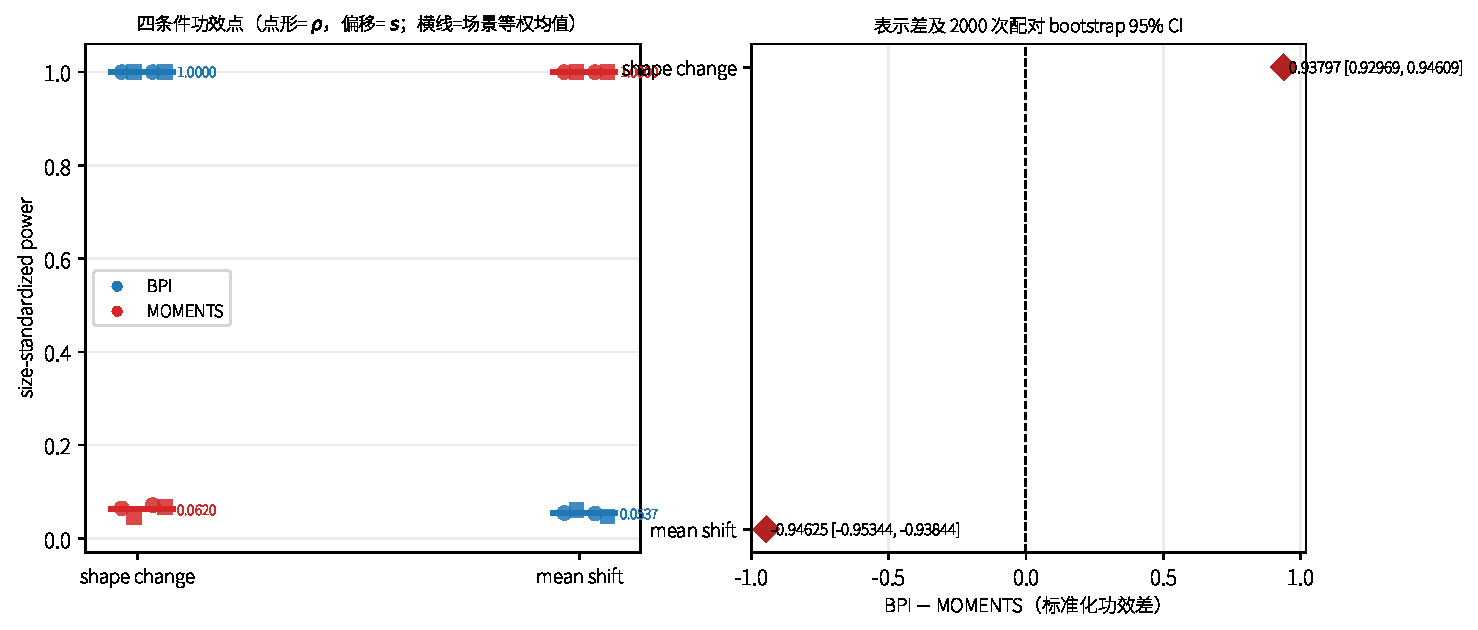
\includegraphics[width=0.95\textwidth]{../artifacts/figures/Figure5_H1_power_and_difference.pdf}
\caption{左：形状变化与均值平移下 BPI 与 MOMENTS 的条件级尺寸标准化功效。小点为四个预设条件之一（点形编码 $\rho$：圆圈 $\rho=0$，方块 $\rho=0.8$；水平偏移编码 $s$）；横线为场景等权平均功效。两个场景之间不使用连线，以避免暗示连续变化趋势。右：两个场景下 BPI 减去 MOMENTS 的功效差及 2000 次配对百分位自助 95\% 区间，零线表示无差异。右图区间只对应表示差异，不用作单个表示功效均值的误差条。完整 16 行条件级结果见补充材料。}\label{fig:h1-power}
\end{figure}

两个场景中出现的样本功效 $1.00000$ 表示 1600 次有限 Monte Carlo 重复在全部四个条件上的汇总结果，未构成总体功效恒等于 1 的概率保证。式\eqref{eq:shape-power-diff}与式\eqref{eq:mean-power-diff}共同支持表示选择性的结论：拓扑表示和矩表示保留了不同类型的变化信息，任何单一表示的检出能力均应结合备择结构加以评价。

\subsection{名义功效与尺寸标准化功效}\label{sec:h1-std}

直接以 $p\le0.05$ 计算的名义功效同时受到观测统计量和校准参考分布的影响。当对应零假设配置未达到点态实用校准时，名义功效可能因反保守性而被抬高，也可能因保守性而被压低。尺寸标准化功效改用匹配零假设统计量的经验临界值，使 BPI 与 MOMENTS 在各自零假设尺度上接受比较。该指标仍是条件化的有限样本量，不能消除表示维数、窗口参数和备择强度等设计因素的影响。

\subsection{定位误差与联合成功率}\label{sec:h1-localization}

位置估计由观测扫描曲线确定，按式\eqref{eq:location-map}映射回原始时间轴。由于变化在 $t=\lfloor T/2\rfloor$ 与 $t=\lfloor T/2\rfloor+1$ 之间发生，真实连续边界为
\begin{equation}\label{eq:true-location}
 \tau_{\mathrm{true}}=\left\lfloor\frac T2\right\rfloor+\frac12.
\end{equation}
本文报告无条件绝对误差
\[
 E_r=|\widehat\tau_r-\tau_{\mathrm{true}}|,
\]
原始尺度平均绝对误差 $R_1^{-1}\sum_rE_r$，以及归一化平均绝对误差
\begin{equation}\label{eq:normalized-mae}
 \operatorname{nMAE}
 =\frac1{R_1}\sum_{r=1}^{R_1}\frac{E_r}{T}.
\end{equation}
位置误差由观测统计量决定，因此对同一“条件--表示”组合，M0 与 M1 共享相同的 $\widehat\tau_r$。校准方法只通过拒绝事件影响联合成功率。对方法 $m\in\{\mathrm{M0},\mathrm{M1}\}$，定义
\begin{equation}\label{eq:joint-success}
 \widehat J_m
 =\frac1{R_1}\sum_{r=1}^{R_1}
 \mathbf1\left\{p_{r,m}\le0.05,\;
 |\widehat\tau_r-\tau_{\mathrm{true}}|\le\frac W2\right\}.
\end{equation}
漏检重复保留在式\eqref{eq:joint-success}的分母中，因此该量同时评价检出与定位。

表~\ref{tab:h1-power}以同一场景内四个预设条件的等权平均汇总功效、归一化定位误差和联合成功率。不同步长对应的 $T$ 不同，故正文采用式\eqref{eq:normalized-mae}保证条件间尺度可比；逐条件原始 MAE、匹配零假设临界值和对应 I 类错误率见补充材料。定位汇总由既有观测扫描结果重新计算，未改变或重跑 Monte Carlo 试次。

\begin{table}[ht]
\centering
\caption{同一场景内四个预设条件的等权描述性汇总。尺寸标准化功效使用各自匹配的零假设临界值；平均归一化 MAE 为无条件位置误差除以对应 $T$ 后的均值；联合成功率按式\eqref{eq:joint-success}分别计算。}\label{tab:h1-power}
\begingroup
\footnotesize
\setlength{\tabcolsep}{3.5pt}
\begin{tabular}{llccrr}
\toprule
场景 & 表示 & 检出能力 & 定位误差 & \multicolumn{2}{c}{检出--定位联合成功}\\
\cmidrule(lr){3-3}\cmidrule(lr){4-4}\cmidrule(lr){5-6}
 & & $\widehat\beta_{\mathrm{std}}$ & nMAE & M0 & M1\\
\midrule
形状变化 & BPI & 1.00000 & 0.00409 & 0.9839 & 0.9839\\
形状变化 & MOMENTS & 0.06203 & 0.20165 & 0.0144 & 0.0009\\
均值平移 & BPI & 0.05375 & 0.20255 & 0.0087 & 0.0011\\
均值平移 & MOMENTS & 1.00000 & 0.00330 & 0.9052 & 0.9052\\
\bottomrule
\end{tabular}
\endgroup
\end{table}


